% \documentclass[]{pnas-new}
\documentclass[9pt,twocolumn,twoside,lineno]{pnas-new}
% Use the lineno option to display guide line numbers if required.
\usepackage{enumitem}


\templatetype{pnasresearcharticle} % Choose template 
% {pnasresearcharticle} = Template for a two-column research article
% {pnasmathematics} %= Template for a one-column mathematics article
% {pnasinvited} %= Template for a PNAS invited submission

\title{Making Community Resilience About People: Measuring Resilience as Access to Services} %Rethinking Resilience: Access to Essentials} %

% Use letters for affiliations, numbers to show equal authorship (if applicable) and to indicate the corresponding author
\author[]{Tom M. Logan}
\author{Seth D. Guikema}
% \author{}

\affil{Industrial and Operations Engineering, University of Michigan, Ann Arbor, USA}

% Please give the surname of the lead author for the running footer
\leadauthor{Logan} 

% Please add here a significance statement to explain the relevance of your work
\significancestatement{
Resilience urgently needs to be operationalized if we are going to prepare our communities for exacerbated natural hazards.
We present and demonstrate a framework that integrates and complements the traditional thinking on community and urban resilience that can provide actionable insight for community decision-makers.
Because essential services such as health care, education, and food are integral to everyday life, we shift the focus onto the accessibility of these services.
In devising this approach we emphasise building equity, addressing vulnerability, and integrating with spatial planning so that our communities are empowered not only to "bounce back" from a disruption, but to "bound forward" and improve the resilience and quality of life for all residents.
}

% Please include corresponding author, author contribution and author declaration information
\authorcontributions{T.L \& S.G devised the approach. T.L collected and analyzed the data, and wrote the paper. Both edited the paper.}
\authordeclaration{The authors declare no conflict of interest.}
\correspondingauthor{\textsuperscript{*}Correspondence should be emailed to tom.logan@canterbury.ac.nz}

% Keywords are not mandatory, but authors are strongly encouraged to provide them. If provided, please include two to five keywords, separated by the pipe symbol, e.g:
\keywords{Community resilience $|$ Natural hazards $|$ Social justice $|$ Spatial planning} 

\begin{abstract}
Despite the extensive discussion surrounding resilience to climate change and natural hazards, operationalizing the concept to enable communities to build their resilience has remained challenging. 
The dominant approaches focus on either evaluating community characteristics or infrastructure functionality. 
While both remain useful, they have several limitations to their ability to provide actionable insight.
Additionally, the current conceptualizations do not consider essential services or how access is impaired by hazards. 
Given that services such as food, education, and healthcare are integral to a community’s well being, access to such services is intrinsic to community resilience. 
We propose a new conceptualization of resilience that is based on access to essential services, together with a way of measuring the resilience of a community based on this conceptualization. 
Using two illustrative examples from the impacts of Hurricanes Florence and Michael, we demonstrate how decision makers and planners can use this framework to visualize and quantify resilience-enhancing interventions and ensure they are equitable. 
\end{abstract}

\dates{This manuscript was compiled on \today}
% \doi{\url{www.pnas.org/cgi/doi/10.1073/pnas.XXXXXXXXXX}}

\begin{document}

\maketitle
\thispagestyle{firststyle}
\ifthenelse{\boolean{shortarticle}}{\ifthenelse{\boolean{singlecolumn}}{\abscontentformatted}{\abscontent}}{}


\dropcap{A}ccess to services is not something we should take for granted, not before nor after a disaster. Following Hurricane Katrina, residents of New Orleans' Lower 9\textsuperscript{th} Ward were forced to take three buses to reach their nearest grocer \cite{Netter2016-dm}. 
The 2017 South Asian floods raised fears that thousands of children permanently dropped out of school \cite{Watt2017-bs}. 
Even without these disasters, many people throughout the world live within food deserts, health care deserts, and without access to other essential services. 
Access to services, such as food, education, healthcare, and culture, is integral for communities to function well \cite{Winter1997-kc, Logan2017-fr, Dempsey2011-og, United_Nations_Educational_Scientific_and_Cultural_Organization2018-sf}.
This makes access to essentials fundamental to community resilience.

Operationalizing resilience is among today's most impactful research questions \cite{Caldarice2019-tv}.
However, resilience is conceptually malleable and multidimensional \cite{Caldarice2019-tv, Meerow2016-definingRes}. 
To capture this complexity, it is widely accepted that no single metric will be sufficient \cite{Bruneau2003-px, Sharma2018-rs, Haimes2009-gj, Levine2014-je, Cutter2014-jm, Cutter2016-landscape}.
We, as a research community, need to develop approaches that complement one another.

% capacity metrics
One existing approach for operationalizing resilience focuses on community capacity. 
Motivating this approach is an understanding that resilience relies on qualities that enable a community to prepare for, respond to, recover from, and improve after hazards \cite{Cutter2014-jm, Zautra2008-rb}.
Indicators are used to quantify these qualities.
These indicators capture aspects including the social, economic, institutional, and infrastructure characteristics \cite{Cutter2014-jm, Cutter2010-vg, Cutter2016-landscape, Sherrieb2010-nk}, and the vulnerability and adaptability of communities \cite{Lam2016-qn}.
This approach is not hazard-specific \cite{Koliou2018-jt}.
Rather, the objective is to determine qualities of a community that can be strengthened to enhance the community's ability to respond and recover \cite{Cutter2014-jm, Cutter2010-vg, Sherrieb2010-nk}. 

% infrastructure functionality
Infrastructure functionality is the other approach.
It focuses on critical infrastructure networks, such as electricity, transportation, communications, potable water, and sewers, with the goal of limiting damage, mitigating the consequences, and hastening the recovery \cite{Bruneau2003-px, Barker2013-od, Hosseini2016-pm, Haimes2009-gj, Guidotti2016-vu, Curt2018-kl}.
Central to this approach is the resilience function or recovery curve, where the network's state (e.g., percent operational) is the focus.
Much of the research in this area has improved how that recovery function is quantified \cite{Bruneau2003-px, Chang2004-et, Cimellaro2010-ov, Vugrin2010-vy, Ayyub2014-mf, Sharma2018-rs}.
Other work has advanced how infrastructure networks can be optimized to reduce their vulnerability or speed their recovery \cite{Hosseini2016-pm, Xu2007-sc}.
On-going advances address the interdependence of the infrastructure to understand how failures may cascade through a system \cite{Guidotti2016-vu, Gardoni2018-xu}.
More recent extensions \cite{Gardoni2018-xu, Clark2018-pr, Guidotti2019-fc} have begun applying the capabilities-approach, which focuses on understanding how hazards affect the opportunities of individuals including being educated and being healthy \cite{Murphy2006-io}. 
This existing work, however, remains focused on the effects from damage to centralized infrastructure.

% limitations
Although these traditional approaches are invaluable for understanding resilience, both have limitations in their ability to provide actionable insight for building resilience.
The indicators of community characteristics remain heavily focused on socio-economic aspects of communities \cite{Koliou2018-jt} and approaches for improvement, such as increasing the community's education, operate on decadal time-scales.
The indicators also often lack validation \cite{Bakkensen2016-ht} and are not intended to provide information regarding how a community responds to a specific hazard or instruction for decision-makers in those cases.
On the other hand, the infrastructure functionality approach is useful for hazard response, but, beyond the hard infrastructure, does not focus on people and their needs \cite{Doorn2018-fx}. 
Until very recently, the approach has ignored the actual people it aims to serve and has remained independent of their needs and vulnerabilities \cite{Cutter2008-placeBasedModel, Cutter2010-vg}.

Neither approach captures how a community can ensure essential services are available to all residents. 
The accessibility of services such as education, healthcare, food, and culture (that critical infrastructure exists to support) is crucial for a community’s vitality, livability, and cohesion \cite{Dempsey2011-og, Talen2003-dc, Winter1997-kc, United_Nations_Educational_Scientific_and_Cultural_Organization2018-sf}. 
Currently our approach to resilience cannot address questions specific to vital community function;
Following a disaster how long must people go without acceptable access to food?

To address the unsolved challenge for community resilience, we need to integrate our understanding of the social system and the physical infrastructure and truly focus on the opportunities for residents \cite{Koliou2018-jt, Cutter2016-landscape}.
Although infrastructure is necessary for many opportunities, it, is not sufficient on its own \cite{Doorn2018-fx}.
Equally, possessing the characteristics of a strong and healthy community is vital, but, alone, is also insufficient.

We offer a fresh perspective on community resilience.
We propose the access to essentials (ATE) resilience framework that integrates and complements the existing approaches to provide actionable insight for communities trying to build their resilience.

\section*{Access to essentials (ATE) resilience framework}

\begin{figure*}
    \centering
    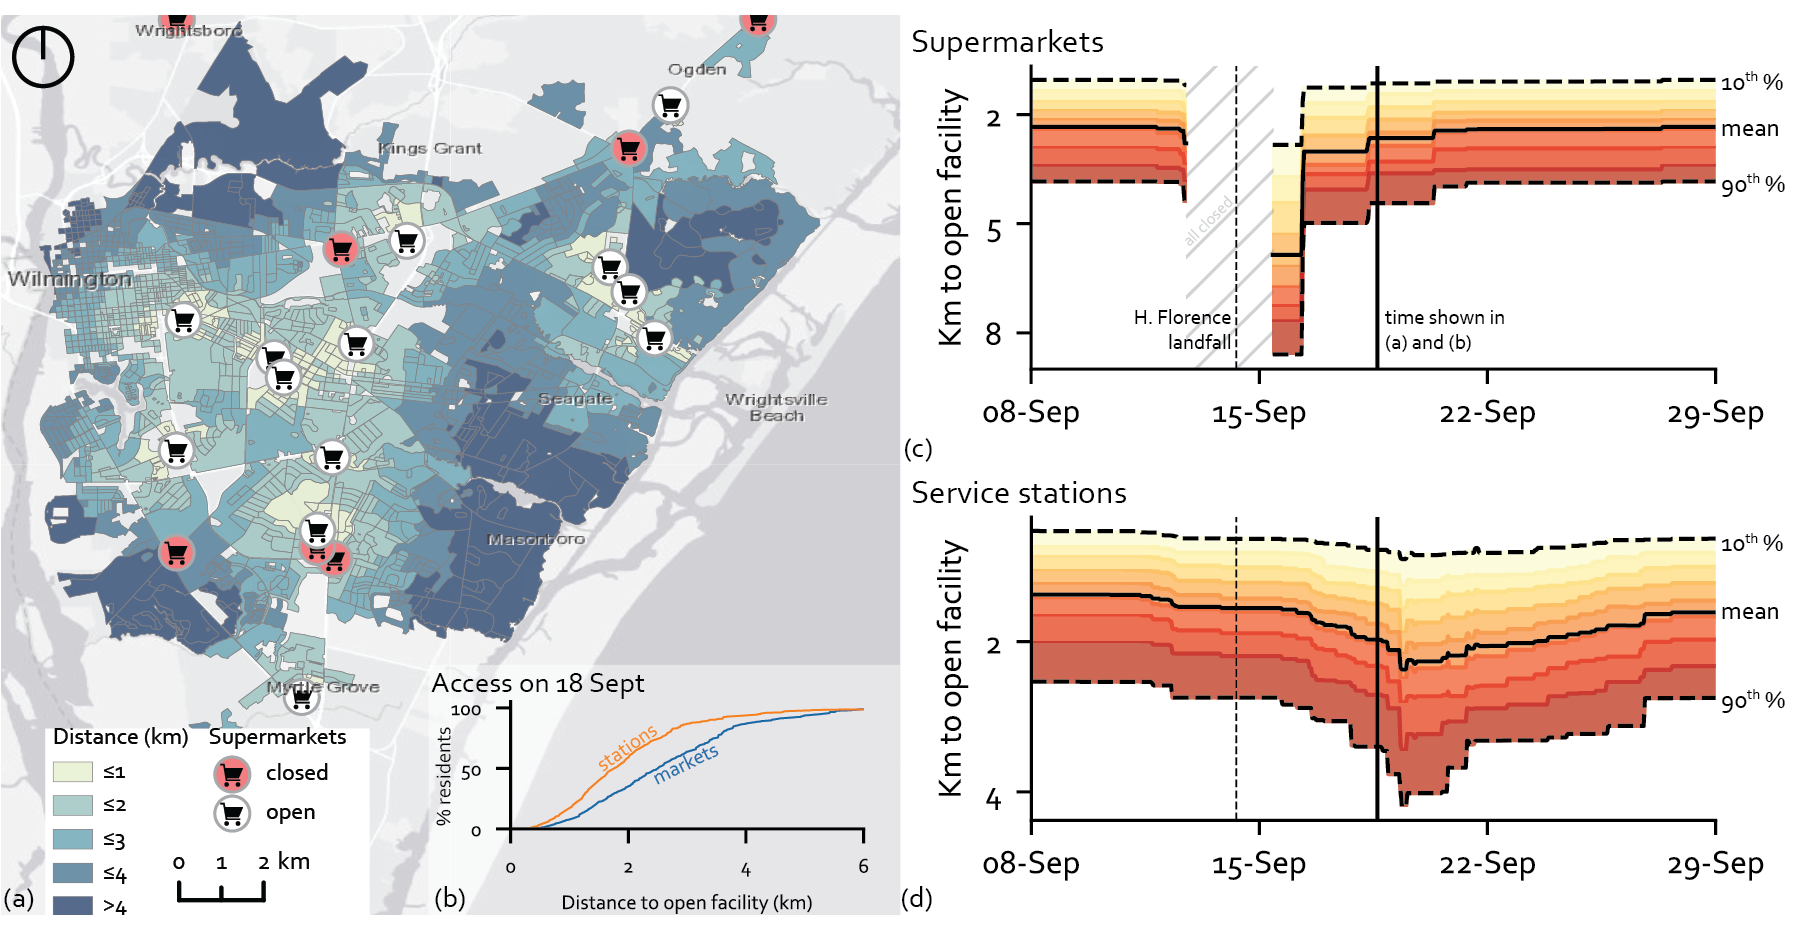
\includegraphics[width=0.8\linewidth]{report/fig/NC_resilience.png}
    \caption{Wilmington, NC on the 18\textsuperscript{th} of September, 2018. (a) The map of distance to nearest operational supermarket for census blocks with non-zero populations, (b) the cumulative distribution function showing the percentage of residents who are closer than $x$ to their nearest operational supermarket and service station, and (c, d) the resilience curves showing how the distribution in access changes over time.
    }
    \label{fig:fig1}
\end{figure*}

ATE measures the distance of residents within a community to their nearest operational essential services. 
As facilities shutter and reopen due to a hazard, we can evaluate what percentage of people are affected, how long it takes to recover, and how the experiences differ across different groups of the population. 
This spatially and temporally explicit approach both 1) identifies where and who requires attention from emergency responders, and 2) encourages interventions to reduce service deserts (e.g., food), both before and after a hazard, to reduce inequity and strengthen the community.

For a specified region, the access to essentials resilience framework involves: 
\begin{enumerate}[topsep=1pt,itemsep=0em,partopsep=1ex,parsep=1ex]
    % \itemsep0em
    \item Engaging the community 
    \begin{enumerate}[topsep=0pt,itemsep=-2pt,partopsep=1ex,parsep=1ex]
        % \itemsep0em
        \item Establish which services are essential, and how needs differ throughout the community
    \end{enumerate}
    \item Measuring accessibility
    \begin{enumerate}[topsep=0pt,itemsep=-2pt,partopsep=1ex,parsep=1ex]
        % \itemsep0em
        \item For each of the essential services, identify the locations of service provision facilities within the region
        \item From each block within the region, determine the network distance to all facilities
        \item For each block, determine the distance to the nearest operational facility
        \item Map the distances to nearest service (Figure \ref{fig:fig1}a)
        \item Plot the distribution of nearest distances (Figure \ref{fig:fig1}b)
    \end{enumerate}
    \item Monitoring the impacts from a hazard
    \begin{enumerate}[topsep=0pt,itemsep=-2pt,partopsep=1ex,parsep=1ex]
        % \itemsep0em
        \item Update the distance to nearest operational services as facilities open and close
        \item Construct the resilience curve showing how residents' access changes over time (Figures \ref{fig:fig1}c, S1)
    \end{enumerate}
    \item Evaluating equality and equity (Figure \ref{fig:equality})
    \begin{enumerate}[topsep=0pt,itemsep=-2pt,partopsep=1ex,parsep=1ex]
        % \itemsep0em
        \item Differentiate residents based on demographics or vulnerability scores
        \item Compare how the access for these various groups changes over time
        \item Identify vulnerable areas to which to provide additional services and improve equity.
    \end{enumerate}
    \item Intervening to build resilience (Figure \ref{fig:haz_cycle})
\end{enumerate}

%%%%%%%%%% How does this integrate the existing methods?
This is a new way of conceptualizing and quantifying community resilience that can support building resilience, independent of the hazard.
ATE can be simulated using both the critical infrastructure and community capacity information.
Critical infrastructure simulation provides ways of estimating which services will not be operational following a hazard.
The community characteristics can be used to evaluate need and assess equity following these simulated disruptions.
In turn, community indicators can be assessed and updated based on these simulations.
Thus, ATE is a resilience framework that integrates the existing approaches with a clear focus on the well-being of the community's residents.

\subsection*{Acceptable access}
\begin{figure}
    \centering
    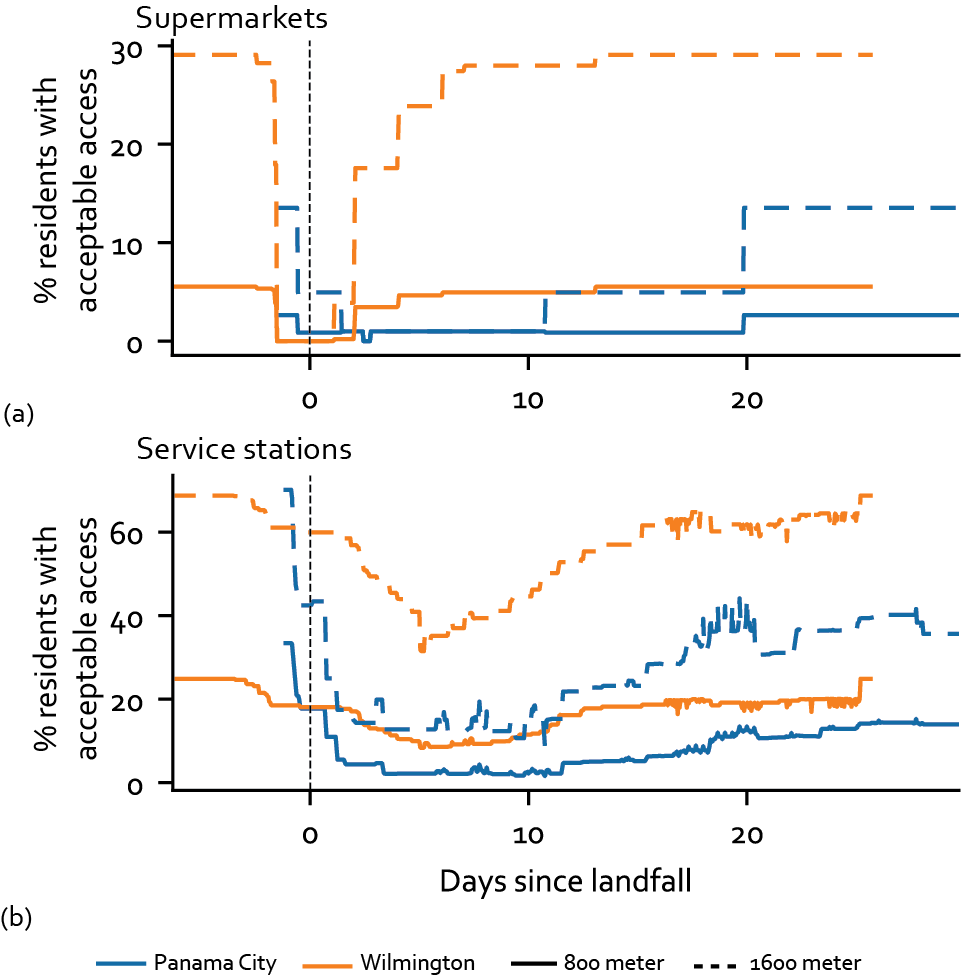
\includegraphics[width=0.8\linewidth]{report/fig/sufficient_only.png}
    \caption{The recovery curves, for Panama City following Michael and Wilmington following Florence, showing the percentage of residents in each city with acceptable access to both (a) supermarkets and (b) service stations. Acceptable access is defined by two distance thresholds. 
    }
    \label{fig:threshold}
\end{figure}

It is possible to specify a minimum acceptable standard for accessibility for each of the services and determine the portion of the community with acceptable access (Figure \ref{fig:threshold}). 
The percentage of the residents with that acceptable access is determined from the cumulative distribution functions (the process is shown in Figure S1). 
The threshold must be place-based and service-specific and determined through community engagement \cite{Pantelic1991-qu, United_Nations_Educational_Scientific_and_Cultural_Organization2018-sf}.

We recognize that while we argue for considering access to essential services as a measure of resilience, we  currently present proximity to services. 
Access, in fact, is comprised of proximity, availability, acceptability, affordability, adequacy, and awareness \cite{Saurman2016-gj, Penchansky1981-qh}. 
Drawing on, and advancing, the relevant literature will lead to the additional dimensions being included for each service. 
These additional dimensions can be included through the use of a metric that defines acceptable access. 
This would specify a minimum level suitable for human well-being \cite{Doorn2018-fx}.
It may even require that proximity, cost, capacity, and other dimensions of accessibility vary based on the characteristics and vulnerabilities of the community to consider social justice (for example, proximity may vary based on car-ownership).
This standard would be normatively indexed, i.e., the standard of acceptability is arbitrary and evolving (analogous to the poverty line, which is geographically specific) \cite{Constas2014-ui}.

Nevertheless, proximity is a necessary component for access to services and provides insight into the resilience of a community. 
A major benefit derived from using proximity, or any continuous measure of access, is the ability to assess the distribution of access across the population. 
There is a very real risk when using thresholds that the residents with extremely poor access, who are often among the most vulnerable, are overlooked because they are aggregated by a binary metric \cite{Logan2017-fr}. 
This is especially important given that poverty lies at the root of disaster vulnerability so true resilience approaches must help correct this \cite{Pantelic1991-qu}.

%%%%%%%%%% Equity and targeting vulnerability
\subsection*{Equality and equity}
\begin{figure}
    \centering
    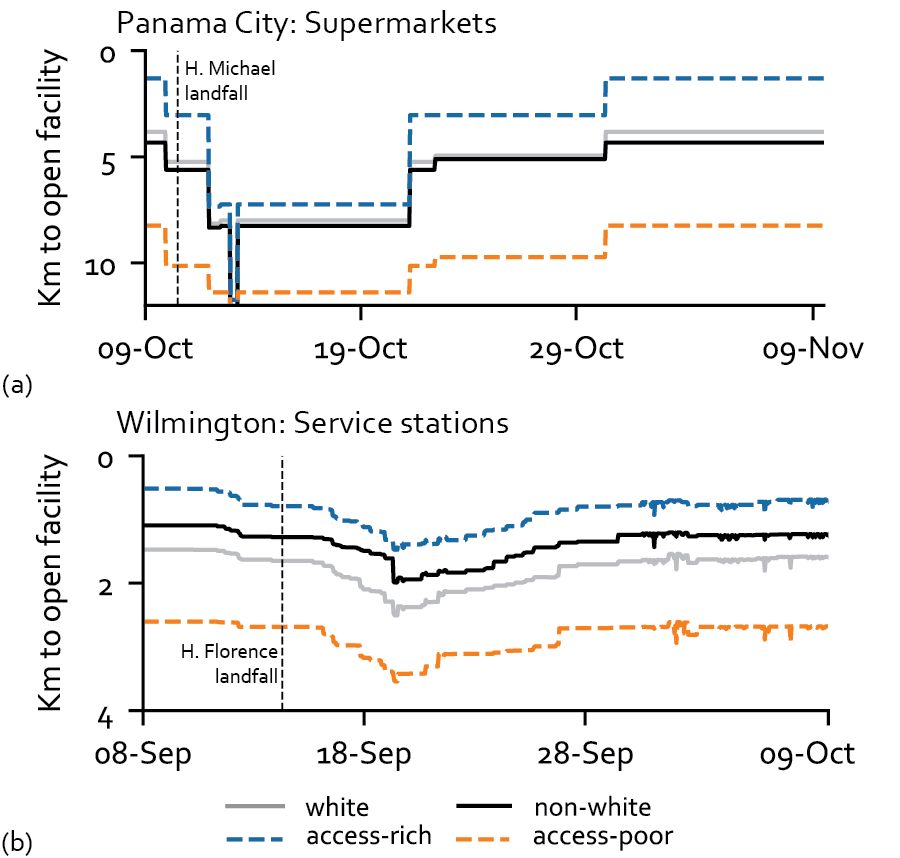
\includegraphics[width=0.8\linewidth]{report/fig/equality.png}
    \caption{Comparing how access to essentials varies between demographic groups and initially access-rich/poor residents (the top and bottom 20\% of residents). This could also be done based on indicators of social vulnerability or community capacity.}
    \label{fig:equality}
\end{figure}
Inequalities may be present before the occurrence of a hazard and are often exacerbated after an event \cite{Gardoni2018-xu}.
ATE can parse different socio-economic characteristics and evaluate the accessibility of services across demographic groups (Figure \ref{fig:equality}) \cite{Williams_undated-sy}.
This allows for needs-based assessments and the integration with indicators of social vulnerability and community capacity.
Potential interventions can be assessed based on how they affect these different groups within the community.

%%%%%%%%%%%% Transformation
\subsection*{Promoting transformation}
The many resilience approaches that prioritize "bouncing back", and quantify resilience using a "change-in functionality", risk further institutionalizing inequity \cite{Normandin2019-hp, I_Sudmeier-Rieux2014-lc, MacKinnon2013-nx}.
Claims such as "residents have grown used to” these abysmal conditions, fail to value the importance of equity and community sustainability for resilience to future events \cite{Dempsey2011-og, Pantelic1991-qu}.
They fail because they do not promote transformation and mitigation that encourages communities to "bound forward."

ATE is deliberately constructed to promote transformation of communities to enhance equity, both before and after a disruption. 
This is achieved primarily in two ways.
First, unlike the critical infrastructure approach, which predominately focuses on the state of infrastructure damage \cite{Cutter2010-vg}, ATE assesses the value residents derive from the system. 
This distinction is important because restoring functionality is not analogous to returning to the previous state e.g., the services can be rebuilt in more desirable spatial configurations.
Second, by assessing actual distance, rather than the difference at any point in time with the initial state ("change-in"), ATE identifies the service-poor residents. 
For example, in Figure \ref{fig:equality}, the largest change in access is experienced by the service-rich residents.
If decisions were made on the basis of this differential, then interventions would be targeted to improve the resilience of service-rich residents, and further exacerbate inequalities.
Instead, decision makers should be aware of pre- and post-hazard service deserts. 
This should mean that both mitigation and reconstruction target and improve the standard of living for all residents \cite{Pantelic1991-qu}. 
This is essential for building sustainable communities, that are enabled to enhance their adaptive capacity and future resilience \cite{Saunders2015-uz}.

\subsection*{Integration with spatial planning}
The existing approaches to resilience are primarily spatially independent.
They do not explicitly require information about a community's layout nor do they support urban planners. 
Integrating land use planning with resilience quantification is essential because spatial planning is among the most effective tools for reducing exposure and sensitivity to extreme events \cite{Brunetta2019-ki, Campbell2006-in, Hurlimann2012-uj} (see \cite{Anderson2018-hr} for climate related examples). 
Surprisingly, there has been little attempt to integrate climate protection and spatial planning in practice \cite{Barnes2017-xf}.
ATE brings spatial planning to the forefront of resilience quantification by clearly linking it with urban changes and social sustainability.
This supports rethinking how our cities are designed, planned, managed, and lived in, in the pursuit of community and urban resilience \cite{Caldarice2019-tv}. 

\section*{Illustrative examples}
\begin{figure*}
    \centering
    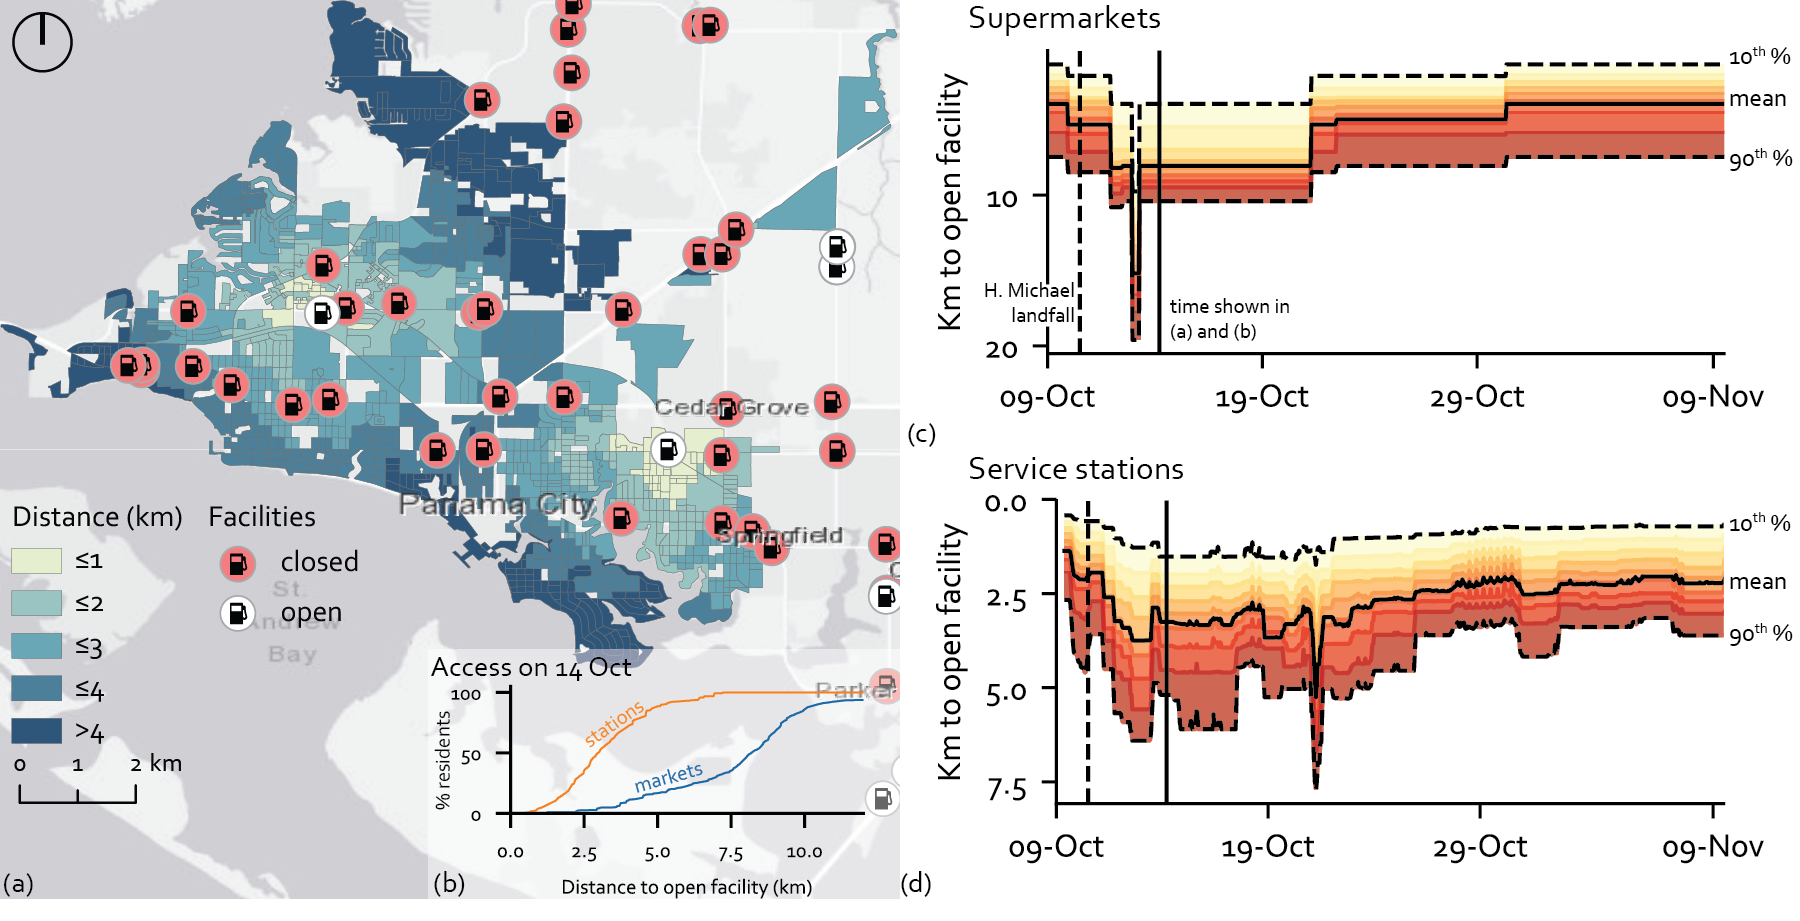
\includegraphics[width=0.8\linewidth]{report/fig/FL_resilience.png}
    \caption{Access in Panama City, FL on the 14\textsuperscript{th} of October, 2018. (a) The map of distance to nearest operational service station, (b) the cumulative distribution function showing how many residents are closer than $x$ to their nearest operational service station and supermarket, and (c, d) the resilience curves showing how the distribution in access changes over time.
    }
    \label{fig:resil_FL}
\end{figure*}
\subsection*{Overview and scope}
We now present two illustrative examples focused on Wilmington, North Carolina, and Panama City, Florida.
In late 2018 they were struck by Hurricanes Florence and Michael respectively. 
The examples demonstrate how the access to two services (grocery stores and service stations) change due to the hurricanes. 
Specifically, we seek to 1) understand the spatial extent of service disruption so service-poor residents can be identified, 2) assess the resilience of the community to these hazards. 
Note that our use of grocery stores and service stations is for demonstration purposes; in practice, determining which services are essential and what distance is acceptable requires community engagement. 

Wilmington, NC is located on the southeastern North Carolina coast.
It has a population of approximately 120,000 people. 
Hurricane Florence made landfall slightly east of Wilmington in the early hours of September 14, 2018, as a Category 1 hurricane. 
Due to the hurricane’s slow movement, it resulted in heavy rainfall beginning September 13, and coupled with strong storm surge, this resulted in heavy flooding. 

By contrast, Panama City, FL, has approximately 37,000 residents and is located along the Emerald Coast of the Florida Panhandle. 
Hurricane Michael made landfall 40km Southeast of Panama City as a Category 4 hurricane on October 10. 
While Florence was notable for its rainfall, Michael caused catastrophic damage due to extreme winds (the strongest in the USA since 1992 with 208 km/h winds) and storm surge. 

\subsection*{Inputs}
For this illustrative example we present the access to grocery stores and service stations before and following the hurricanes. 
Service locations were determined using GasBuddy\footnote{https://tracker.gasbuddy.com} and supermarkets were identified manually using Google Maps.
Access to these services was calculated at the US census block (neighborhood block) level and shapefiles and demographic data was sourced from IPUMS \cite{Manson2018-ug}. 
The Open Street Map street network was downloaded from Geofabrik\footnote{http://download.geofabrik.de/}. 
The distance from each block to all services was calculated using the Open Source Routing Machine using the approach described in Logan et. al \cite{Logan2017-fr}. 
Facility closure was recorded from GasBuddy, Twitter, and the supermarket websites.

\subsection*{Results}
Figures \ref{fig:fig1}, \ref{fig:resil_FL}, S2 \& S3 show access in Wilmington and Panama City following the hurricanes. 
The maps can be used to identify service-deserts and the recovery functions show how quickly the cities restore access and how acceptable that access is.

As an example, there appears to be a food-desert in western Wilmington \ref{fig:fig1}a, so these residents may require emergency food supplies even after the other stores reopen.
Note that due to data availability, the supermarket results do not include all food outlets as we only obtained information for stores that were reporting their opening times.
Although these results do not comprehensively present food-deserts, they provide a demonstration of using this approach.
These maps could be varied to highlight sectors of the community with high social vulnerability, or, for example, a higher proportion of aged residents, so that emergency response can target need.

Recovery times and access quality are shown in Figures \ref{fig:fig1}c,d, \ref{fig:resil_FL}c,d, and \ref{fig:threshold}. 
Supermarkets appear to reopen faster than service stations, likely due to resources provided by their parent companies.
In Wilmington, this was a matter of days.
Access to service stations in Wilmington was still deteriorating by the time supermarket access was almost restored (Figures \ref{fig:fig1} \& \ref{fig:threshold}).
This is likely due to failures in the supply chains.
However, inventory information was unavailable to us for supermarkets.

In Panama City, the recovery took significantly longer for both supermarkets and service stations (Figure \ref{fig:threshold}).
However, this comparison does not reflect differences between the cities' resilience, because the hurricanes were different. 
Nevertheless, it is clear that Panama City suffered more and for longer.

In both cities, the access to supermarkets is less than desirable (Figure \ref{fig:threshold}).
Even before the hurricanes, only 30\% of residents in Wilmington live within 1 mile (1600 meters) and this is further than the majority of distance thresholds considered acceptable (e.g., \cite{Talen2003-dc}).
In Panama City this worse still, but the results are skewed due to our omission of some food stores that would be included in practice.
Regardless, this shows that there are likely service-deserts existing within the cities that could be mitigated prior to a hazard.

\section*{Application throughout the hazard cycle}
\begin{figure}
    \centering
    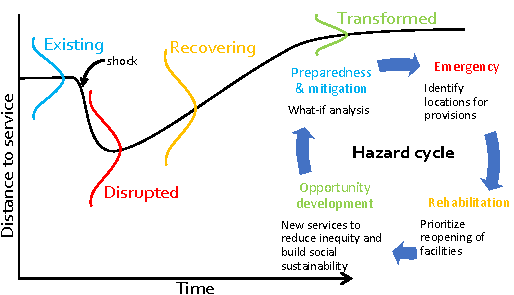
\includegraphics[width=\linewidth]{report/fig/Figure_hazardCycle.pdf}
    \caption{This resilience function (aka recovery curve) shows how the access, and its distribution, may change before, during, and after a hazard. The hazard cycle shows how the ATE resilience framework can be utilized by decision-makers from mitigation to recovery.}
    \label{fig:haz_cycle}
\end{figure}
ATE can enhance decision making throughout the hazard management cycle. 
The cycle (Figure \ref{fig:haz_cycle}) involves preparing for and mitigating potential hazards; emergency response; and recovery, including the immediate rehabilitation and longer term (re)construction: opportunity development.

Implementing this framework in the field will require real-time information about the functioning of services.
For example, local networks or reporting systems could be implemented.
This, coupled with improvements in proximity analysis \cite{Logan2017-fr, noel2019-pypi}, mean that essential service access can be evaluated before, during, and after a hazard strikes.
This can be used to guide emergency response as well as short-term and long-term recovery and development. 

\subsection*{Mitigation and preparedness}
Before any hazard occurs, existing inequities to service-deserts should be addressed.
This will enhance community cohesion and social capital \cite{Dempsey2011-og} and enable residents to utilize all opportunities \cite{Cutter2010-vg}.
Additionally, "what-if" simulation can determine which facilities are critical in servicing the community. 
This type of analysis can be used to build redundancy or robustness into the system \cite{Wardekker2010-hw}.

\subsection*{Emergency response}
During and immediately following a disruption, ATE enables responders to identify impacted areas and allocate resources appropriately. 
Updating the service accessibility map in real-time supports targeting supplies like food and health care to places in need. 
Based on population characteristics, vulnerabilities and needs could be considered so that situations such as the ignoring of vulnerable residents in the Rockaways, NY, following Hurricane Sandy \cite{Subaiya2014-qx}, do not reoccur. 

\subsection*{Rehabilitation} 
During this phase, short term and basic essential services are restored \cite{Resendiz-Vazquez2019-ol}. 
Facility reopening can be coordinated and optimized to maximize accessibility. 
Other amenities, perhaps recreational or spiritual \cite{United_Nations_Educational_Scientific_and_Cultural_Organization2018-sf} (although amenity importance is community and culture specific), can be prioritized for reopening in the same manner.

\subsection*{Opportunity development}
We should build back better \cite{Resendiz-Vazquez2019-ol} by not only enhancing protection against future hazards \cite{Platt2019-lx}, but by improving equity and residents’ quality of life \cite{Pantelic1991-qu}. 
This latter phase of recovery is referred to as “opportunity development” rather than "re"construction \cite{Resendiz-Vazquez2019-ol,Pantelic1991-qu}. 
In this phase, urban planning must be leveraged to encourage desired amenities such as grocery stores to establish in certain locations. 
For example, comprehensive plans can be used to set minimum numbers for food retailers, zoning mechanisms can simplify the regulatory process, and subsidies or other incentives can recruit retailers to in-need areas \cite{Raja2010-cm, Raja2008-wx}. 

\section*{Conclusion}
The urgent need for communities to build their resilience means that operationalizing resilience is among today's most impactful research questions and practical challenges \cite{Caldarice2019-tv}.
While there has been significant work on resilience, the existing approaches are limited in the actionable insight they provide.
No resilience measure currently focuses on the provision of everyday amenities such as food, health care, and education, which are vital for residents to participate in life.
The access to essentials (ATE) resilience framework that we propose integrates key aspects of the traditional approaches to resilience and complements their use with the goal of maintaining, restoring, and improving equitable access to essential services.

ATE provides a spatially explicit approach to quantifying resilience of access to services with a direct focus on people's well-being. 
It involves measuring the access of residents to the services and monitoring how that access changes before, during, and after a hazard event. 
Critical to our framework is the ability to discern how access changes between different demographics and vulnerable groups within a community.
Equally important is that we've devised the framework in a way that promotes continuous improvement of access to all residents and transforming the system, rather than bouncing back to pre-event conditions.
ATE has utility during all phases of the hazard cycle by providing actionable information to decision makers from preparation to post-event improvement.
By being spatially explicit, ATE integrates resilience quantification with urban planning, which is crucial for our society's response to evolving threats exacerbated by climate change.

To end-users, we reiterate that while this approach is adaptable and scalable, resilience is place-based and therefore community specific, so the application of this framework must succeed community engagement and understanding.

Rethinking resilience as access to essential services promotes bounding forward, rather than bouncing back. It complements and integrates aspects of both dominant existing approaches to community resilience. We encourage transformation by shifting the focus from the state of infrastructure to the value it provides to people. This naturally enhances adaptive capacity of the community and existing capacity indicators can be used to prioritize vulnerable residents. The access to essentials framework formalizes resilience in a way that enables and encourages communities to build their resilience equitably. 

% \matmethods{\subsection*{Data}
% We use the Centers for Disease Control and Prevention's (CDC's) 500 cities data 

% }
% \showmatmethods{} % Display the Materials and Methods section

\acknow{We would like to acknowledge funding for this work provided by a University of Michigan Rackham PreDoctoral Fellowship, the US National Science Foundation (grant 1638197), and One Concern Inc. (through a grant to the U. of Michigan). All opinions expressed in this paper are our own.}

\showacknow{} % Display the acknowledgments section

% Bibliography
\bibliography{references.bib}

\end{document}